%\hl{Internet of Things (IoT) refers to a system of connected physical objects via the internet. The 'thing' in IoT can refer to a person or any device which is assigned through an IP address. A 'thing' collects and transfers data over the internet without any manual intervention with the help of embedded technology. It helps them to interact with the external environment or internal states to take the decisions.}

%The proliferation of the Internet of Things (IoT) is fostering the connection of massive numbers of devices to the network. It is predicted that by 2020 there will be 50 to 100 billion devices connected to the Internet and constantly producing data[].

%IoT analytics refers to the analysis of data from multiple IoT data sources, including sensors, actuators, smart devices and other internet connected objects. The collection and analysis of data streams from IoT sources is nowadays considered a key element of the IoT’s disruptive power, as well as a prerequisite to realizing IoT’s hyped market potential. Indeed, according to a recent report by McKinsey[], less than 1\% of IoT data is currently used, which is a serious set-back to maximizing IoT’s business value. For example, most IoT analytics applications are nowadays used for anomaly detection and control rather than for optimization and prediction, which are the applications that will provide the greatest business value in the coming years.

%\section{IoT Data and BigData}

%\hl{Big data means a large set (petabytes or gigabytes) of structured, unstructured or semi-structured data and analyzing those data to get the insights of the business trend.}


%\section{Challenges of IoT Applications}

%Internet of Things(IoT) and big data are closely intertwined and although they are not the same thing.
%The term big data existed long before IoT arrived. When the information demonstrates veracity, velocity, variety and volume, then it is interpreted as big data

%IoT data is essentially BigData since they feature several of the Vs of BigData, including
%\begin{itemize}
%    \item Volume: IoT data is machine-generated data coming from a wide variety of sensors, where big data is mostly human-generated data.
%    \item Velocity: Refers to the speed data is being produced, collected and analyzed. IoT, data needs to ingest hundreds of thousands, or even millions, of events per second from their devices.
%    \item Variety: Since IoT encompasses a large variety of IoT devices, IoT data can be very heterogeneous both in terms of semantics and data formats.
%    \item Veracity: Several IoT streams are noisy and incomplete, which creates uncertainty in the scope of IoT analytics applications. Statistical and probabilistic approaches must be therefore employed in order to take into account the noisy nature of IoT data streams, especially in cases where they stem from unreliable sensors.
%\end{itemize}

%IoT data differ from big data datasets and introduces new challenges, this are some of the new characteristics that IoT introduces:

%\begin{itemize}
%    \item Data heterogeneity:
%    \item Real-time nature: While in big data projects it is perfectly normal for data to rest before it is used in any kind of analysis, in any IoT projects time is of the absolute essence, for several application must be processes nearly in real-time.
%    \item Time and location dependencies: IoT data is naturally geo-distributed and generated at the edge of the network, sometimes involving fast moving sensors. Big data is mostly generated from a single location, the core of the network.
%    \item Privacy and security sensitivity:
%\end{itemize}

%\section{IoT Application Lifecycle}
%The IoT application lifecycle comprises of the following three phases: Data Collection, Data Analysis and Data Storage and Query.

%\begin{enumerate}
%\item \textbf{Data collection:} gathers data from multiple sources and brings them to the pipeline.
%\item \textbf{Data Analysis:} processes the data and performs computations on the collected data.   
%\item \textbf{Data Storage and Query:} reads and writes data to the main memory and disk.
%\end{enumerate}

The Internet of Things (IoT) is an emerging concept that is fostering the connection of massive numbers of objects, sensors, and devices to the network. As per Cisco systems\footnote{Cisco, Internet of Things At-a-Glance, 2016 }, 500 billion devices are expected to be connected the Internet by 2030, and nearly half of the worldwide data will come from sensors~\cite{McAuley}. 
%
IoT devices produce important and timely data that can lead to new and transformative applications that are important to science and society, such as:
%
\begin{itemize} 
  \item Precision medicine applications that benefit from runtime actuation based on continuous monitoring by scientific instruments.
  \item Urban mobility applications that rely on processing data from sensors to identify and alleviate traffic congestion. 
  \item Healthcare applications that infer lifestyle patterns based on behavioral information obtained from wearables. 
\end{itemize} 

Making such applications a reality requires collecting data from sensors and instruments, processing this data individually or collectively in a timely manner, and making decisions based on the results. 

Stream processing frameworks (SPFs) have proven to be very effective at processing large amounts of data at near-real time, especially when combined with the elasticity and scalability of the cloud. Nonetheless, existing solutions were developed keeping in mind Big Data streams generated at the core of the infrastructure, such as those associated with web analytics. As a result, applying these solutions to IoT data stream requires transferring data from the edges to a data center located at the core of the infrastructure for processing. The prevalent model of moving data located at the edge of the network to the core of the network to process is quickly becoming unsustainable~\cite{intro}. The resulting impact on latency, network congestion, storage cost, and privacy can limit the potential impact of IoT.

However, in recent years, non-trivial computational capabilities have proliferated across the computing service landscape~\cite{continuum}. In particular, edge services are emerging close to the data sources and can provide potential data-processing capabilities\cite{dastjerdi2016fog,bonomi2014fog}. Furthermore, not all the data produced is interesting or relevant, and only a part of it may need to be processed in the context of an application. These observations can be leveraged to design hybrid architectures that can effectively leverage both the edge and the cloud resources to process the data in an effective and timely manner\cite{ahmed2017role, satyanarayanan2015edge}.

Although the cloud is better suited to perform heavier (resource intensive) analysis, such as processing historical events and very large datasets, edge devices can support real-time analytics that consider the temporal, spatial, and continuous nature of IoT data. 

While such edge-based data processing can benefit IoT applications, edge resources are typically constrained in their capabilities. Therefore, the edge resources can be leveraged to complement the computing capabilities of the cloud-centric approach and reduce the overall latency and bandwidth requirements. The use of the edge and cloud architecture poses the following challenges: 

\begin{itemize}
\item Deciding how to split such IoT applications among the edge and cloud resources;

\item Exploring heterogeneous infrastructure for deploying dataflow applications has proved to be NP-hard \cite{Benoit:2013}.
 
\item Moving operators from cloud to edge devices is challenging due to the devices' limitations with respect to memory, CPU, and often network bandwidth \cite{dias:2018:survey}.
\end{itemize}

Solving the challenges presented above in a correct manner will allow for faster completion time, a reduction in edge to cloud data transfers, and ensure an efficient use of the edge and cloud resources. Doing them incorrectly can be detrimental to throughput and exacerbate the time for handling data events.
 
Such flexibility is not currently offered in state-of-the-art IoT systems or stream processing engines. Major systems, such as Azure IoT~\cite{azure}, AWS Greengrass~\cite{amazon}, and IBM Watson IoT~\cite{IBM}, do not offer programming support for orchestrating the execution of data-processing tasks between the cloud and the edge. Therefore, the developers' ability to specify ``What data needs to be processed?,'' ``Where to deploy the computations?,'' and ``When to deploy the computations?,'' is limited. Moreover, existing IoT stacks tend to perform poorly when deployed on constrained devices, making it nearly impossible to support real-time data analytics on these devices.


\section{Motivation}

Due to the proliferation of the Internet of Things (IoT) paradigm, the number of devices connected to the Internet is growing. These devices are generating unprecedented amounts of data at the edges of the infrastructure. Although the generated data provides great potential, identifying and processing relevant data points hidden in streams of unimportant data, and doing this in near real time, remains a significant challenge. Existing stream processing platforms require the data to be transported to the cloud for processing, resulting in latencies that can prevent timely decision making or may reduce the amount of data processed.

To address these limitations, we propose R-Pulsar, a software stack with a content- and location-based programming abstraction to perform and orchestrate data analytics between the edge and the cloud. The programming abstraction enables developers to address the \textbf{what}, \textbf{where}, and \textbf{when} data needs to be processed by specifying content and action descriptors. We also propose a programming model to provide developers with the ability to define \textbf{how} to automatically split the dataflow across the edge and the cloud by specifying a set of dataflow constraints. In addition we present an optimized data-processing pipeline for achieving real-time data analytics on constrained devices.


\section{Problem Description}


\section{Contributions}
The primary contributions of the research in this thesis are a programming model for deciding \textbf{what}, \textbf{when}, \textbf{where} data needs to be processed by specifying content and action descriptors and \textbf{how} computations get distributed across the edge and the cloud. The detailed contributions are presented as follows.
\begin{itemize}
  \item A content- and location-based programming abstraction for specifying \textbf{what} data gets collected and \textbf{where} the data gets analyzed.
  \item A rule-based programming abstraction for specifying \textbf{when} to trigger data-processing tasks based on data observations.
  \item A programming abstraction for specifying \textbf{how} to split a given dataflow and place operators across edge and cloud resources.
  \item An operator placement strategy that aims to minimize an aggregate cost which covers the end-to-end latency (time for an event to traverse the entire dataflow), the data transfer rate (amount of data transferred between the edge and the cloud) and the messaging cost (number of messages transferred between edge and the cloud).
  \item Performance optimizations on the data-processing pipeline in order to achieve real-time performance on constrained devices.
  \item An implementation of the above capabilities as part of the R-Pulsar software stack and its evaluation using embedded devices (Raspberry Pi and Android phone).
\end{itemize}

\section{Outline}

\begin{figure}[h!]
  \centering
  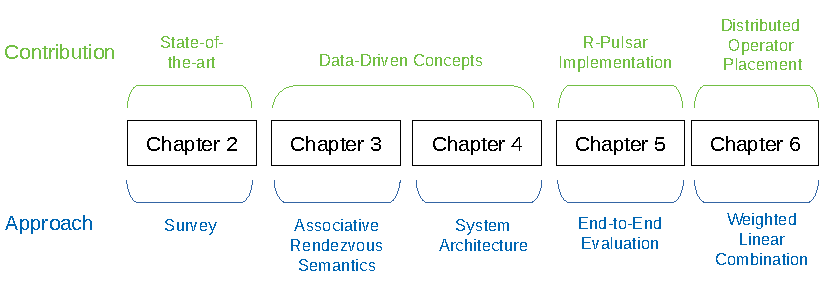
\includegraphics[width=1\textwidth]{Figures/Outline.pdf}
  \caption{Thesis Organization.}
  \label{fig:Outline}
\end{figure}

The core chapters of the thesis are structured as shown in Figure~\ref{fig:Outline} and are deviated from articles and journals published during the PhD. The remaining of the thesis is organized as follows: 

\begin{itemize}
    \item Chapter 2 shows the motivating use cases that where used to build R-Pulsar. 
    \item Chapter 3 presents an extensive literature review of related work. 
    \item Chapter 4 presents the programming abstraction that R-Pulsar builds upon.
    \item Chapter 5 presents the system concepts on what R-Pulsar was build upon. 
    \item Chapter 6 presents the implementation and evaluation details of R-Pulsar. 
    \item Chapter 7 introduces the operator placement problem. 
    \item Chapter 8 concludes the dissertation by outlining future research work.
\end{itemize}

